\subsection{Solving the DE}
We can solve these differential equation through separation of variables:

\textbf{Case 1: }
From 1 we have:

\begin{align*}
    -k &= m \frac{dv}{dt}
    \\ \int -k dt &= \int m dv
    \\ -kt &= mv + c_1
    \\ \Aboxed{v &= \frac{-kt - c_1}{m}}
\end{align*}

\textbf{Case 2:}
From 2 we have: 

\begin{align*}
    -k - F_b &= m \frac{dv}{dt}
    \\ \int -k - F_bdt &= \int mdv
    \\ -kt - F_b &= mv + c_2
    \\ \Aboxed{v &= \frac{-kt-F_bt-c_2}{m}}
\end{align*}

\subsection{Justification of parameters chosen}
After carefully examining the data, I have chosen that the brakes were applied when t=9s. I choose t=9s to be the time when the brakes were applied as the gradient of the graph seems to decrease drastically after t=9, and this can easily be observed from the change of shape from the graph. From this we can deduce that the initial conditions are:
%Draw graph to show the gradient decreases rapidly after t=10
\\ \\
\textbf{Case 1: } t = 0s, v = 96ms\textsuperscript{-1} and t=9s, v=55ms \textsuperscript{-1}
\\
\textbf{Case 2: } t = 9s, v = 55ms\textsuperscript{-1} and t=26s, v=0ms \textsuperscript{-1}
\\ \\
So using this, we can see that the first model will give us a function of velocity from 0 to 9s, and model 2 will give us a function of velocity that will model the velocity from 9s until the aeroplane comes to a complete stop, which is at t=26s. Both models use the point (t=9, v=55), as not using this point would result in the graph being discontinuous, and thus not an accurate model of what is happening. Also, having a continuous graph is necessary as it will be crucial when finding the area under the graph in order to find the length of the runway required for the aeroplane.

\subsection{Solutions of the DE}
\textbf{Case1: } 
Using the initial conditions, we can find v as a function of t
\\ \\
Using the point (t=0, v=96), we see that:
\begin{center}
\begin{align*}
    v &= \frac{-kt - c_1}{m}
    \\ 96 &= \frac{-c_1}{m}
    \\ \d c_1 &= -96m
\end{align*}
\end{center}
Using the point (t=9, v=55), we see that:
\begin{center}
\begin{align*}
    v &= \frac{-kt - c_1}{m}
    \\ 55 &= \frac{-9k+96m}{m}
    \\ 55m &= -9k + 96
    \\ 9k &= 41m
    \\ k &= \frac{41}{9}m
    \\ &= 4.56m
\end{align*}
\end{center}

From this we can deduce that for case 1:

\begin{equation}
    \boxed{v = -4.56t + 96}
\end{equation}

\textbf{Case 2: } 
Using the initial conditions, we can find v as a function of t
\\ \\
Using the point (t=9, v=55), we see that:
\begin{center}
\begin{align*}
    v &= \frac{-kt-F_bt-c_2}{m}
    \\ v &= -\frac{-41t}{9}t - \frac{F_bt - c_2}{m}
    \\ 55 &= -41 - \frac{9F_b}{m} -\frac{c}{m}
    \\ 96 &= -\frac{9F_b}{m} - \frac{c_2}{m}
\end{align*}
\end{center}
Using the point (t=26, v=0), we see that:
\begin{center}
\begin{align*}
    v &= \frac{-kt-F_bt-c_2}{m}
    \\ v &= -\frac{-41t}{9} - \frac{F_bt - c_2}{m}
    \\ 0 &= -\frac{1066t}{9} - \frac{26F_b}{m} -\frac{c_2}{m}
\end{align*}
\end{center}
\begin{equation}
     \frac{1066m}{9} = -26F_b - c_2
\end{equation}

Therefore by solving the simultaneous equation we find:
\begin{align*}
    F_b &= -\frac{8080000}{51}
    \\ &= -158431.3725
    \\ c_2 &= -\frac{171600000}{17}
    \\ &= -10094117.65
\end{align*}

Therefore we can conclude that for case 2:
\begin{equation}
    \boxed{v = -3.24t + 84.1}
\end{equation}

\subsection{Model Performance}
By using the solutions, that we found we can make a prediction for every value of t. Once we have made the predictions, we can then find the error using the RMS error. The RMS error is calculated using the formula $\sqrt{\sum{\frac{1}{27}(v_{actual} - v_{predicted})^2}}$ or by using the formula $\sqrt{\sum{\frac{1}{27}(d_i)^2}}$ . Once the RMS is calculated it can be used to compare the performance of the model, and how it compares to the other improved models.
\\ \\
\begin{table}[H]
\centering
    \begin{tabular}{|l|l|l|l|l|l|l|l|l|l|l|l|l|l|l|l|l|}
        \hline
        t(s) & 0 & 1 & 2 & 3 & 4 & 5 & 6 & 7 & 8 & 9 \\ \cline{1-11} 
        predicted v(m/s) & 96.00 & 91.44 & 86.89 & 82.33 & 77.78 & 73.22 & 68.67 & 64.11 & 59.56 & 55.00\\ \cline{1-11}
        Actual v(m/s) & 96 & 89 & 82 & 77 & 72 & 68 & 64 & 61 & 58 & 55 \\ \cline{1-11}
        $d^2$ & 0.00 & 5.98 & 23.90 & 28.44 & 33.38 & 27.27 &	21.78 & 9.68 & 2.42 & 0.00 \\ \cline{1-11}
    \end{tabular}
    \caption{Case 1}
    \vspace{0.5cm}
    
    \begin{tabular}{|l|l|l|l|l|l|l|l|l|l|l|l|}
        \hline
        t(s) & 10 & 11 & 12 & 13 & 14 & 15 & 16 & 17 & 18 \\ \cline{1-10}
        predicted v(m/s) & 51.76 & 48.53 & 45.29 & 42.06 & 38.82 & 35.59 & 32.35 & 29.12 & 25.88 \\ \cline{1-10}
        Actual v(m/s) & 50 & 46 & 41 & 38 & 34 & 31 & 27 & 24 & 21 \\ \cline{1-10}
        $d^2$ & 3.11 & 6.40 & 18.44 & 16.47 & 23.27 & 21.05 & 28.65 & 26.19 & 23.84 \\ \cline{1-10}
    \end{tabular}
    \caption{Case 2}
    \vspace{0.5cm}
    
    \begin{tabular}{|l|l|l|l|l|l|l|l|l|}
        \hline
        t(s) & 19 & 20 & 21 & 22 & 23 & 24 & 25 & 26 \\ \cline{1-9}
        predicted v(m/s) & 22.65 & 19.41 & 16.18 & 12.94 & 9.71 & 6.47 & 3.24 & 0.00 \\ \cline{1-9}
        Actual v(m/s) & 18 & 16 & 13 & 10 & 8 & 5 & 3 & 0
        \\ \cline{1-9}
        $d^2$ & 21.60 & 11.64 & 10.09 & 8.65 & 2.91 & 2.16 & 0.06 & 0.00 \\ \cline{1-9}
    \end{tabular}
    \caption{Case 2 continued}
    \vspace{0.5cm}
\end{table}

\begin{figure}[H]
\centering
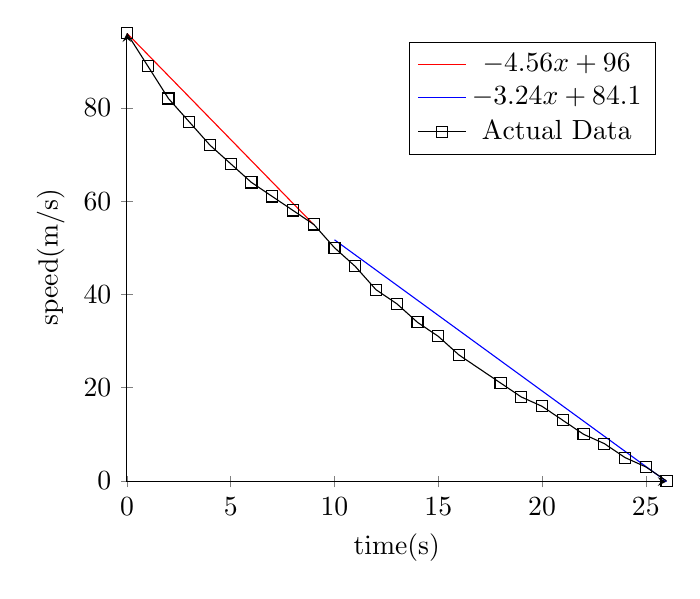
\begin{tikzpicture}
\begin{axis}[
    axis lines = left,
    xlabel = time(s),
    ylabel = speed(m/s),
]
%Below the red parabola is defined
\addplot [
    domain=0:9,
    samples=100, 
    color=red,
]
{-4.56*x + 96};
\addlegendentry{$-4.56x + 96$}
%Here the blue parabloa is defined
\addplot [
    domain=10:26, 
    samples=100, 
    color=blue,
    ]
    {-3.24*x + 84.1};
\addlegendentry{$-3.24x + 84.1$}
 
 \addplot[
    color=black,
    mark=square]
    coordinates {(0,96)(1,89)(2,82)(3,77)(4,72)(5,68)(6,64)(7,61)(8,58)(9,55)(10,50)(11,46)(12,41)(13,38)(14,34)(15,31)(16,27)(18,21)(19,18)(20,16)(21,13)(22,10)(23,8)(24,5)(25,3)(26,0)};
\addlegendentry{Actual Data}
\end{axis}
\end{tikzpicture}
\caption{Graph showing the predicted velocity values against the actual velocity values}
\end{figure}